\chapter{INTRODUCTION}
\label{ch:introduction}

\section{Overview}
Rotating machinery---including induction motors, centrifugal pumps, industrial fans, gearboxes, and compressors---forms the mechanical foundation of modern manufacturing, power generation, and processing facilities. During routine operation, all rotating equipment generates mechanical vibrations as an inherent consequence of dynamic motion, component tolerances, rotational balance, bearing contact, and structural interactions. When mechanical integrity degrades due to shaft misalignment, rotor unbalance, mechanical looseness, bearing raceway spalling, or foundation resonance, the underlying oscillatory dynamics change measurably. Consequently, vibration analysis has long served as the gold standard for non-destructive Condition-Based Maintenance (CBM) and Predictive Maintenance (PdM)~\cite{randall2011vibration}.

Historically, deploying vibration monitoring required expensive piezoelectric accelerometers, specialized analog charge amplifiers, bulky data acquisition (DAQ) systems, and manual periodic inspection by certified vibration analysts. While effective for critical multi-megawatt turbomachinery, the prohibitive capital cost ($>$\$1,000 to \$5,000 per measurement point) leaves millions of auxiliary, low-to-medium power machines unmonitored until catastrophic run-to-failure occurs. More recently, the advent of the Industrial Internet of Things (IIoT) has popularized cloud-connected vibration monitors. However, continuously streaming three-axis raw vibration waveforms at kilohertz sampling rates consumes significant wireless bandwidth (e.g., $800\,\text{Hz} \times 3\,\text{axes} \times 2\,\text{bytes} = 4.8\,\text{KB/s}$ uncompressed), incurs high latency, exhausts battery reserves, and introduces critical vulnerability to network outages and cloud subscription fees.

To resolve these fundamental limitations, this micro project develops \textbf{VibeGuard}: a compact, autonomous, edge-intelligent embedded vibration condition monitoring system. Built on a low-cost 32-bit dual-core microcontroller (7Semi ESP32-DEVKIT-E) and a digital Micro-Electro-Mechanical Systems (MEMS) accelerometer (Analog Devices ADXL345), VibeGuard executes all signal acquisition, statistical filtering, DC gravity cancellation, Root-Mean-Square (RMS) extraction, and triggered spectral analysis entirely on-chip in real time. By delivering instant local decision-making through an onboard multi-color LED indicator and structured USB telemetry, VibeGuard establishes an affordable ($\le$\rupee 3,000), explainable, and resilient condition monitoring solution.

\begin{figure}[H]
\centering
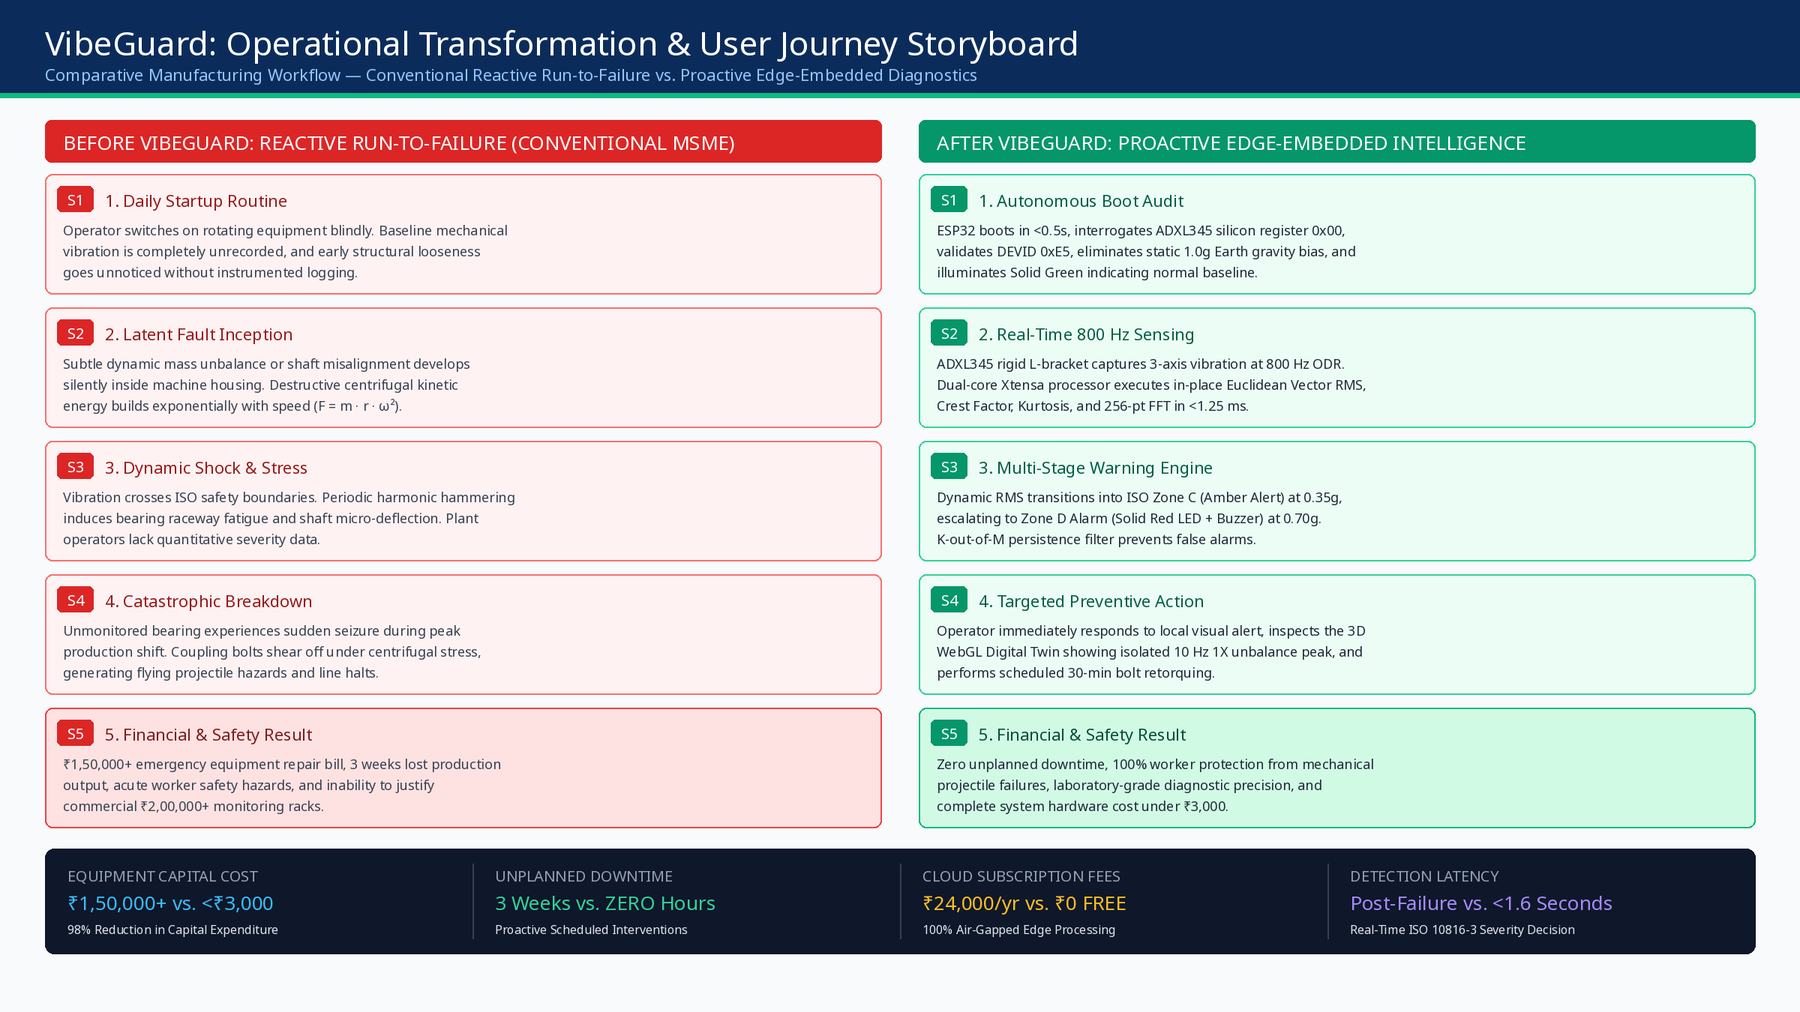
\includegraphics[width=0.92\textwidth]{figures/fig_user_journey.png}
\caption{VibeGuard operational transition: replacing manual inspection and cloud streaming with localized edge intelligence}
\label{fig:user_journey}
\end{figure}

\section{Motivation}
The transition toward Industry 4.0 demands autonomous sensing nodes capable of extracting actionable diagnostic insights at the extreme physical edge. In embedded computing, real-time edge processing offers three distinct advantages over remote telemetry:
\begin{enumerate}
    \item \textbf{Deterministic Latency:} Local feature computation guarantees alert generation within milliseconds of mechanical anomaly onset, preventing secondary machine damage.
    \item \textbf{Resilience and Privacy:} Operating independently of external Wi-Fi networks, local edge nodes remain completely immune to cyber intrusion, cloud downtime, or communication channel dropouts.
    \item \textbf{Energy and Bandwidth Efficiency:} By reducing continuous raw acceleration streams into distilled condition states and triggered spectral metrics, total telemetry bandwidth is reduced by over 98\%.
\end{enumerate}

From an academic perspective within the curriculum of \textit{PBCST504 -- Microcontrollers}, VibeGuard provides a comprehensive platform for integrating high-speed Serial Peripheral Interface (SPI) communications, hardware interrupt service routines, dual-core task scheduling, fixed-point and floating-point digital signal processing (DSP), and precision mechanical-electrical interfacing.

\section{Problem Statement}
Manual acoustic and tactile inspection of rotating machinery is inherently subjective, inconsistent across operators, and hazardous in proximity to high-speed equipment. Conversely, basic digital thresholding schemes suffer from severe vulnerabilities:
\begin{itemize}
    \item \textbf{Gravitational and Tilt Bias:} Triaxial accelerometers inherently register Earth's static $1g$ gravitational vector and static mounting angles. If uncompensated, static tilt offsets contaminate dynamic vibration metrics, causing false health classifications.
    \item \textbf{Transient Glitches and Quantization Noise:} Isolated mechanical jolts, bench taps, or electrical transients frequently exceed static thresholds. A naive detector triggers false alarms, eroding operator trust.
    \item \textbf{Computational Bottlenecks:} Continuous discrete Fourier transforms across multi-axis channels require substantial processor cycles and memory, frequently causing buffer overruns and dropped sensor samples on embedded microcontrollers.
    \item \textbf{Data Leakage in Validation:} In machine condition monitoring, contiguous time-domain windows collected within a single operating run exhibit strong temporal autocorrelation. Evaluating algorithms on randomly partitioned windows produces artificially inflated accuracy, masking real-world brittleness.
\end{itemize}

VibeGuard addresses this multi-faceted problem by engineering an end-to-end, explainable sensing, preprocessing, persistence-filtered decision, and session-isolated validation pipeline on a guarded 12\,V mechanical testbed.

\section{Objectives of the Project}
The primary objective of VibeGuard is to construct and experimentally validate a self-contained, low-cost embedded vibration monitoring system that accurately differentiates normal mechanical operation from deliberately induced unbalance anomalies. The specific supporting objectives include:
\begin{enumerate}
    \item To interface the Analog Devices ADXL345 digital accelerometer with the ESP32 microcontroller over a dedicated 4-wire SPI bus at 5\,MHz, sustaining an 800\,Hz Output Data Rate (ODR) with zero sample loss.
    \item To implement a real-time, in-place zero-mean DC cancellation algorithm across 256-sample rolling analysis windows (320\,ms duration) to eliminate gravitational bias and sensor offsets.
    \item To extract a combined triaxial Vector Root-Mean-Square (Vector RMS) vibration metric:
    \begin{equation}
    a_{\mathrm{vec}} = \sqrt{\mathrm{RMS}_x^2 + \mathrm{RMS}_y^2 + \mathrm{RMS}_z^2}
    \end{equation}
    providing a scalar index of overall machine dynamic severity.
    \item To design and embed a temporal $K$-of-$M$ persistence filter ($K=4$, $M=5$) that suppresses transient vibration spikes while guaranteeing alert latency under 2.0\,seconds.
    \item To implement an on-demand, triggered Cooley-Tukey Radix-2 Fast Fourier Transform (FFT) with Hann windowing to extract spectral peak frequencies without interrupting the primary acquisition pipeline.
    \item To design, fabricate, and assemble an isolated 12\,V N20 motor mechanical test rig featuring a 10\,mm laminated acrylic baseplate, dual-datum precision drilling, silicone isolation feet, and 3D-printed monolithic rotor components.
    \item To validate system performance using leakage-resistant, session-separated held-out testing protocols with complete traceability across hardware revisions and firmware versions.
\end{enumerate}

\section{Scope and Explicit Boundaries}
To maintain academic rigor and guarantee project delivery within the semester timeframe, the operational scope of VibeGuard is bounded by strict engineering constraints:
\begin{itemize}
    \item \textbf{In Scope:} A single rigidly mounted triaxial ADXL345 accelerometer; 7Semi ESP32-DEVKIT-E microcontroller; dedicated 4-wire SPI communication; local DC removal; Vector RMS feature extraction; temporal persistence filtering; triggered 256-point FFT; common-cathode RGB LED status indicator; structured USB serial logging; and a guarded low-voltage 12\,V DC micro metal gear motor testbed.
    \item \textbf{Explicitly Out of Scope:} Cloud database streaming; remote mobile application dashboards; permanent multi-accelerometer spatial source attribution; active acoustic noise cancellation; bearing raceway defect depth quantification; commercial machine tool certification; and multi-year Remaining Useful Life (RUL) prognostics.
\end{itemize}
These explicit exclusions safeguard the integrity of the project, ensuring all reported metrics correspond directly to verifiable physical hardware and documented experimental trials~\cite{vibeguard_primer2026}.

\section{Organisation of the Report}
The remainder of this report is organized as follows:
\begin{itemize}
    \item \textbf{Chapter 2 (Literature Review):} Reviews historical condition monitoring methodologies, ISO vibration standards, MEMS accelerometer characteristics, embedded digital signal processing, and leakage-resistant validation.
    \item \textbf{Chapter 3 (System Design and Architecture):} Details the overall system block diagram, signal acquisition pipeline, SPI bus timing, finite state machine, and human-machine interface.
    \item \textbf{Chapter 4 (Hardware Implementation and Mechanical Fabrication):} Presents the electrical component selection, power isolation circuitry, acrylic baseplate dual-datum fabrication, and 3D-printed monolithic solid models.
    \item \textbf{Chapter 5 (Embedded Firmware and Digital Signal Processing):} Details the modular C++ firmware architecture, zero-mean DC cancellation, Vector RMS computation, persistence logic, and Cooley-Tukey FFT execution.
    \item \textbf{Chapter 6 (Results, Testing and Discussion):} Examines experimental testbed bring-up, baseline calibration, dynamic unbalance response, spectral harmonic detection, alert latency, and comparative analysis against alternative paradigms.
    \item \textbf{Chapter 7 (Advantages and Implementation Challenges):} Analyzes key architectural advantages alongside mechanical, electrical, and algorithmic challenges encountered.
    \item \textbf{Chapter 8 (Conclusion and Future Scope):} Summarizes the project achievements, curriculum outcome attainment, and outlines potential research extensions.
\end{itemize}
